\documentclass[11pt,a4paper]{article}
\usepackage{iftex}
\ifXeTeX
  \usepackage{fontspec}
\else
  \usepackage[utf8]{inputenc}
  \usepackage[T1]{fontenc}
\fi
\usepackage[provide=*,french]{babel}
\usepackage[a4paper,margin=2.2cm,headheight=14pt]{geometry}
\usepackage{graphicx}
\usepackage{booktabs}
\usepackage{array}
\usepackage{enumitem}
\usepackage{xcolor}
\usepackage[most]{tcolorbox}
\usepackage{fancyhdr}
\usepackage{titlesec}
\usepackage{longtable}
\usepackage{amsmath,amssymb}
\usepackage[colorlinks=true,linkcolor=cBleu,urlcolor=cBleu,citecolor=cBleu]{hyperref}

\definecolor{cBleu}{RGB}{31,59,99}
\definecolor{cOr}{RGB}{217,161,59}
\definecolor{cRouge}{RGB}{176,58,46}
\definecolor{cVert}{RGB}{60,120,80}
\definecolor{cGris}{RGB}{90,90,90}

\providecommand{\ier}{\textsuperscript{er}}
\providecommand{\iere}{\textsuperscript{re}}
\providecommand{\ieme}{\textsuperscript{e}}

\titleformat{\section}{\Large\bfseries\color{cBleu}}{\thesection}{0.6em}{}
\titleformat{\subsection}{\large\bfseries\color{cBleu!80!black}}{\thesubsection}{0.6em}{}
\titlespacing*{\section}{0pt}{1.6em}{0.7em}

\pagestyle{fancy}
\fancyhf{}
\fancyhead[L]{\footnotesize\color{cGris}Projet Python pour la data science — lobbies et travail législatif}
\fancyhead[R]{\footnotesize\color{cGris}\thepage}
\renewcommand{\headrulewidth}{0.3pt}

\newtcolorbox{encadre}[1][]{enhanced,colback=cBleu!4,colframe=cBleu,
  title={#1},fonttitle=\bfseries,breakable,left=4pt,right=4pt,top=4pt,bottom=4pt}
\newtcolorbox{alerte}[1][]{enhanced,colback=cRouge!4,colframe=cRouge,
  title={#1},fonttitle=\bfseries,breakable,left=4pt,right=4pt,top=4pt,bottom=4pt}
\newtcolorbox{bon}[1][]{enhanced,colback=cVert!5,colframe=cVert,
  title={#1},fonttitle=\bfseries,breakable,left=4pt,right=4pt,top=4pt,bottom=4pt}
\newtcolorbox{jargon}[1][]{enhanced,colback=gray!7,colframe=gray!55!black,
  title={#1},fonttitle=\bfseries,breakable,left=4pt,right=4pt,top=4pt,bottom=4pt}

\newcommand{\chiffre}[1]{\textcolor{cBleu}{\textbf{#1}}}
\newcommand{\fichier}[1]{\texttt{\small #1}}
\setlist[itemize]{itemsep=2pt,topsep=3pt,leftmargin=1.3em}
\setlist[enumerate]{itemsep=2pt,topsep=3pt,leftmargin=1.5em}
\setlength{\parskip}{0.45em}
\setlength{\parindent}{0pt}
\renewcommand{\arraystretch}{1.15}
% Absorbe les débordements de ligne plutôt que de laisser dépasser dans la marge.
\setlength{\emergencystretch}{3em}
\hbadness=10000
\sloppy


\begin{document}

\begin{titlepage}
\centering
\vspace*{2.2cm}
{\color{cBleu}\rule{\textwidth}{2pt}}\\[0.6em]
{\Huge\bfseries\color{cBleu} Cartographier l'influence déclarée\\[0.25em] des lobbies sur le travail législatif\par}
\vspace{0.5em}
{\color{cBleu}\rule{\textwidth}{2pt}}\\[1.6em]
{\Large Ce que contient le projet, comment il a été construit,\\[0.3em] et ce qu'il faut en retenir\par}
\vspace{2.2cm}
{\large Projet évalué du cours \textbf{Python pour la data science}\\[0.3em]
ENSAE 2A --- \texttt{CSC\_4CS08\_AE}\par}
\vspace{1.4cm}
\begin{minipage}{0.84\textwidth}
\color{cGris}\small
Trois sources officielles croisées pour une seule question : la présence déclarée de
lobbies sur un texte de loi laisse-t-elle une trace observable dans le travail et les
votes des députés ? Ce document raconte le projet de bout en bout --- les données, la
méthode, les erreurs commises et corrigées, les résultats, et ce qu'il reste à faire.
Il n'est pas le rendu : le rendu est le dépôt GitHub et son notebook. Il est là pour
que tu saches exactement ce que tu rends.
\end{minipage}
\vfill
{\color{cGris}\small Document généré le \today\par}
\end{titlepage}

\tableofcontents
\newpage

% =====================================================================
\section{En une page}

\begin{encadre}[L'essentiel]
\textbf{La question.} Est-ce qu'on voit, dans les amendements et les votes des députés,
la trace des lobbies qui déclarent avoir travaillé sur un texte de loi ?

\textbf{Les données.} Environ \chiffre{700~Mo}, quatre producteurs publics, aucune
authentification : \chiffre{113\,075} activités de lobbying déclarées à la HATVP,
\chiffre{1\,273\,091} votes nominatifs de députés, \chiffre{126\,392} amendements,
\chiffre{11\,438} intérêts déclarés par les députés, et la population de
\chiffre{34\,955} communes pour mesurer la ruralité des circonscriptions.

\textbf{La difficulté.} Les trois bases n'ont \emph{aucune clé commune}. Le répertoire
des lobbies ne cite jamais de numéro de texte, ne donne pas de date précise, et ne nomme
jamais le député approché. Tout le projet consiste à construire ce lien --- et surtout à
\emph{mesurer à quel point il est faux}.

\textbf{Les résultats.}
\begin{enumerate}
\item Sur le \textbf{vote final}, la discipline de groupe explique tout : la règle
  « chacun vote comme son bloc » se trompe sur \chiffre{3 votes sur 547} pour la loi
  agricole. Il n'y a rien de plus à expliquer à ce niveau.
\item Sur les \textbf{votes d'amendements}, où 4,3~\% des positions s'écartent du groupe,
  la proximité avec les demandes des lobbies va dans le sens attendu mais
  \textbf{n'est pas significative} ($p \approx 0{,}08$), et le reste pour toutes les
  variantes testées.
\item Sur l'\textbf{adoption des amendements}, aucun effet non plus --- mais le test
  témoin, lui, est significatif, ce qui apprend quelque chose sur la mesure.
\item Le seul résultat \textbf{bien identifié} ne concerne pas les lobbies mais les
  députés : déclarer un intérêt privé dans le secteur d'un texte multiplie par
  \chiffre{1,7 à 3,0} la probabilité d'y déposer un amendement.
\end{enumerate}

\textbf{Ce qui fait la valeur du projet.} Pas les résultats, qui sont pour l'essentiel
négatifs. Le travail de rapprochement des bases, et sa \emph{mesure} : 99,5~\% de
précision sur un rattachement interne à l'Assemblée, 100~\% sur 20~paires relues à la
main pour le ciblage des lobbies --- contre 6~\% pour la règle qu'on avait écrite
d'abord. Le résultat méthodologique le plus solide est négatif :
\emph{une règle de rapprochement plausible peut être fausse neuf fois sur dix, et seule
une relecture manuelle le révèle.}
\end{encadre}

\subsection*{Où est quoi}

\begin{center}
\begin{tabular}{@{}p{0.34\textwidth}p{0.6\textwidth}@{}}
\toprule
\textbf{Chemin} & \textbf{Ce que c'est} \\
\midrule
\fichier{notebooks/rapport.ipynb} & \textbf{Le rendu.} Le rapport académique, 92 cellules,
s'exécute en moins d'une minute sans erreur. \\
\fichier{src/lobbynomics/} & Le code, neuf modules, un par étape du raisonnement. \\
\fichier{docs/methode.md} & Le détail méthodologique et toutes les limites. \\
\fichier{docs/sources.md} & Provenance, licences, pièges de chaque source. \\
\fichier{docs/journal.md} & Journal de bord : décisions, erreurs, prochaines étapes. \\
\fichier{data/raw/} & Les 700~Mo de sources brutes (hors Git, retéléchargeables). \\
\fichier{reports/figures/} & Les 18 figures. \\
\fichier{tests/} & 58 tests. \\
\bottomrule
\end{tabular}
\end{center}

Tout se relance par une commande : \fichier{make pipeline}.

\newpage
% =====================================================================
\section{Le sujet, et pourquoi il tient debout}

\subsection{La question posée}

Le lobbying parlementaire est documenté par la presse mais rarement mesuré. Depuis 2017,
la France dispose pourtant d'un \textbf{répertoire des représentants d'intérêts} : toute
organisation qui cherche à influencer une décision publique doit s'y déclarer et décrire
ses actions. En parallèle, l'Assemblée nationale publie en open data l'intégralité de ses
scrutins nominatifs et de ses amendements.

L'idée du projet est de croiser les deux. Pas pour « prouver la corruption » --- ce serait
indéfendable avec ces données, et le dire clairement fait partie du travail --- mais pour
\textbf{cartographier une influence déclarée} : est-ce que la présence affichée de lobbies
d'un secteur sur un texte se voit dans le contenu des amendements et le sens des votes,
une fois qu'on tient compte de l'appartenance politique ?

\subsection{Les quatre textes retenus}

Couvrir toute l'Assemblée n'aurait aucun sens. On s'est restreint à quatre textes de la
XVII\ieme{} législature, choisis parce que le lobbying y est documenté et les volumes
suffisants.

\begin{center}
\small
\begin{tabular}{@{}llrrr@{}}
\toprule
\textbf{Clé} & \textbf{Texte} & \textbf{Scrutins} & \textbf{Amend.} & \textbf{Lobbies} \\
\midrule
\texttt{agriculture} & Loi d'urgence pour la souveraineté agricole & 422 & 1\,592 & 29 \\
\texttt{defense} & Actualisation de la programmation militaire & 292 & 572 & 14 \\
\texttt{fraudes} & Lutte contre les fraudes sociales et fiscales & 262 & 747 & 165 \\
\texttt{logement} & Mobilisation de l'habitat existant & 23 & 68 & \textbf{0} \\
\bottomrule
\end{tabular}
\end{center}

La dernière colonne compte les activités de lobbying qui \emph{nomment} le texte. Le
quatrième texte en a zéro, alors que 419 activités lui sont thématiquement proches : il
sert de \textbf{cas témoin} et n'entre pas dans la modélisation. On y revient
section~\ref{sec:niveaux}, c'est l'argument le plus économique du projet.

\begin{jargon}[Vocabulaire : trois mots qui reviennent partout]
\textbf{Scrutin} --- un vote de l'Assemblée, identifié par un numéro. Un même texte de loi
donne lieu à des centaines de scrutins (un par amendement mis aux voix, plus le vote sur
l'ensemble).\\[2pt]
\textbf{Dossier législatif} --- le « dossier » d'un texte de loi dans la nomenclature de
l'Assemblée. C'est l'identifiant qu'on cherche à retrouver partout.\\[2pt]
\textbf{Activité (au sens HATVP)} --- une action de lobbying déclarée par une organisation :
un objet en texte libre, un domaine, une année. C'est l'unité de base du répertoire.
\end{jargon}

\newpage
% =====================================================================
\section{Les données}

\subsection{Ce qui a été téléchargé}

\begin{center}
\small
\begin{tabular}{@{}p{0.27\textwidth}rp{0.49\textwidth}@{}}
\toprule
\textbf{Source} & \textbf{Volume} & \textbf{Ce qu'on en tire} \\
\midrule
Répertoire HATVP des représentants d'intérêts & 139~Mo & 4\,094 organisations,
\chiffre{113\,075} activités déclarées : objet, domaine, type de décideur visé \\
Déclarations des responsables publics (HATVP) & 83~Mo & 2\,570 déclarations de députés,
\chiffre{11\,438} intérêts : anciens employeurs, participations, bénévolat \\
Scrutins publics, Assemblée & 26~Mo & 8\,455 scrutins, \chiffre{1\,273\,091} votes nominatifs \\
Amendements, Assemblée & 304~Mo & \chiffre{126\,392} amendements avec exposé des motifs \\
Dossiers législatifs & 11~Mo & 2\,971 dossiers, titres et fenêtres de débat \\
Acteurs, mandats, organes & 14~Mo & 649 députés, groupes, commissions, \emph{et le lien
vers leur fiche HATVP} \\
API Géo (Etalab) & 4~Mo & 34\,955 communes : population et surface, pour mesurer la ruralité \\
\bottomrule
\end{tabular}
\end{center}

Tout est public et sans clé d'API. Un \textbf{manifeste} est écrit à chaque collecte
(\fichier{data/raw/\_manifeste.json}) : il enregistre pour chaque fichier son URL, sa
taille, une empreinte SHA-256 et l'horodatage. C'est lui qui permet de dire \emph{quelle
version} des données a produit les résultats --- une source open data change sans prévenir.

\begin{alerte}[Trois pièges rencontrés, qui coûtent une demi-journée chacun]
\begin{itemize}
\item L'URL officielle des amendements est \fichier{amendements\_div\_legis}, pas
  \fichier{amendements\_legis} : la seconde renvoie une erreur~404 silencieuse.
\item \fichier{liste.csv} de la HATVP n'est \emph{pas} le répertoire des lobbies : c'est
  l'index des déclarations des élus. Les deux sont régulièrement confondus.
\item Le JSON de l'Assemblée est une conversion automatique de XML. Un champ absent peut
  valoir \texttt{null}, \texttt{\{"@xsi:nil": "true"\}} ou \texttt{\{"\#text": "…"\}} ; une
  liste d'un seul élément devient un dictionnaire. Deux fonctions du code
  (\texttt{\_txt} et \texttt{\_liste}) n'existent que pour absorber ça, et sont couvertes
  par des tests.
\end{itemize}
\end{alerte}

\subsection{Les contrôles de qualité}

Une erreur de lecture de fichier produit une exception, qu'on voit tout de suite. Une
erreur de \emph{données} produit un tableau plausible et faux, qu'on ne voit jamais. Le
module \fichier{quality.py} écrit donc noir sur blanc ce qu'on attend des tables et
vérifie que c'est vrai : identifiants uniques, intégrité entre tables, cohérence des
décomptes de votes, plages de dates. \chiffre{24 contrôles}, tous au vert aujourd'hui.

Une première version en signalait trois en rouge. Les trois se sont révélées être des
\textbf{régularités explicables} --- et c'est la raison pour laquelle ce sont devenus des
contrôles précis plutôt que des seuils génériques :

\begin{center}
\small
\begin{tabular}{@{}p{0.42\textwidth}p{0.52\textwidth}@{}}
\toprule
\textbf{Anomalie apparente} & \textbf{Explication trouvée} \\
\midrule
44,5~\% des amendements sans « sort » & un amendement n'a de sort que s'il a été
\emph{discuté} : la relation est exacte, pas approximative \\
1,1~\% des amendements sans auteur & ce sont exactement les amendements du
\textbf{Gouvernement}, qui n'a pas d'auteur député \\
12 scrutins pointant vers un dossier introuvable & leurs identifiants commencent tous par
\texttt{DLR5L16} : des textes entamés sous la législature \emph{précédente} \\
\bottomrule
\end{tabular}
\end{center}

Quatre lignes résistaient encore à la deuxième explication : des amendements à l'état
« effacé », dont l'auteur a été retiré en même temps que le contenu. Quatre sur 126\,392 ---
mais quatre lignes inexpliquées suffisent à faire douter du reste, donc elles sont
tracées et exclues explicitement.

\newpage
% =====================================================================
\section{Le problème central : aucune clé commune}

C'est le cœur du projet, et c'est ce que le correcteur regardera.

\begin{center}
\small
\begin{tabular}{@{}lllp{0.2\textwidth}@{}}
\toprule
& \textbf{Unité} & \textbf{Identifiant du texte} & \textbf{Date} \\
\midrule
Scrutins & un vote & présent \textbf{une fois sur trois} & au jour \\
Amendements & un amendement & toujours présent & au jour \\
Répertoire HATVP & une activité & \textbf{aucun} --- du texte libre & à l'année \\
\bottomrule
\end{tabular}
\end{center}

Le répertoire ne dit pas « j'ai travaillé sur le dossier DLR5L17N54085 ». Il dit :

\begin{center}
\itshape\small « Défendre les loups dans le cadre de la loi d'urgence agricole »
\end{center}

Relier les deux est une \textbf{inférence}, pas une jointure. La bonne question n'est donc
pas « comment faire le lien » mais « quelle est la probabilité que ce lien soit faux ».

\subsection{Premier rapprochement : un scrutin et son dossier}

Sur 8\,455 scrutins, \chiffre{5\,826} n'ont aucun lien explicite vers leur dossier. Mais
leur titre nomme le texte :

\begin{center}
\small\itshape
« l'amendement n\textsuperscript{o}~190 de M.~Golliot après l'article~2 de la
\textbf{proposition de loi visant à la nationalisation d'ArcelorMittal France}
(première lecture). »
\end{center}

On extrait la dénomination, on la compare aux titres des 2\,971 dossiers par similarité de
chaînes, et --- c'est l'étape qui fait tout --- on \textbf{arbitre par la date}.

\begin{bon}[Comment la précision est passée de 95,7~\% à 99,5~\%]
La première version s'arrêtait à la similarité de titre et plafonnait à 95,7~\%. En
relisant les erreurs une par une, le motif saute aux yeux : \textbf{l'Assemblée ouvre un
dossier distinct par lecture}. « Nationalisation d'ArcelorMittal France » existe
\emph{deux fois} dans la base. Un score de similarité de 100 ne départage alors rien.

En gardant tous les candidats à moins de 3 points du meilleur, puis en retenant celui dont
la fenêtre d'activité parlementaire est la plus proche de la date du scrutin, la précision
passe à \chiffre{99,5~\%}.
\end{bon}

Le point méthodologique important : ce taux d'erreur est \textbf{mesuré, pas estimé}. Les
2\,608 scrutins qui portent \emph{déjà} un lien explicite forment une vérité terrain
gratuite. On leur applique quand même la méthode approximative et on compare.

\begin{figure}[htbp]
\centering
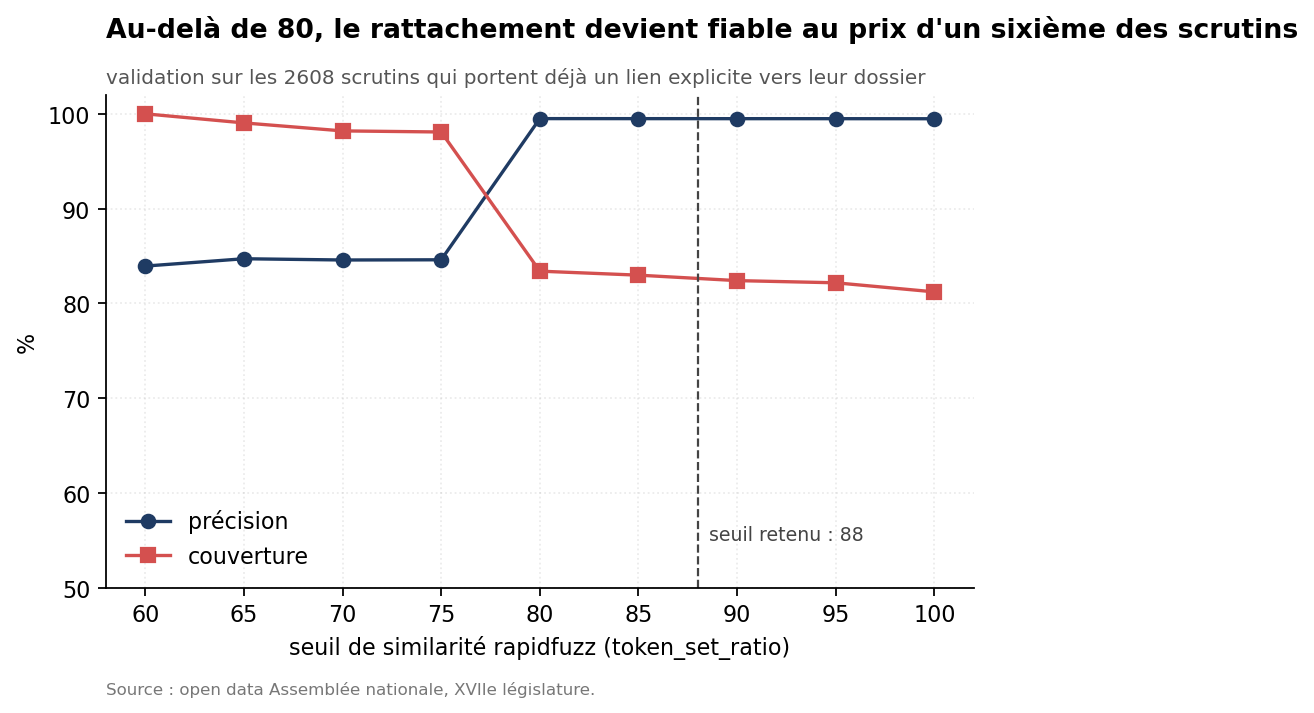
\includegraphics[width=0.84\textwidth]{../reports/figures/01_qualite_matching.png}
\caption{La marche entre les seuils 75 et 80 est franche : en dessous, on rattache des
textes seulement voisins. Le seuil retenu (88) coûte un sixième des scrutins, et c'est un
coût assumé et chiffré plutôt qu'un sixième de lignes fausses.}
\end{figure}

Bilan : \chiffre{90,7~\%} des scrutins rattachés (2\,629 par lien déclaré, 5\,041 par
similarité). Les 9,3~\% restants sont des titres qui ne nomment aucun texte
(« l'ensemble du texte »).

\newpage
\subsection{Second rapprochement : une activité de lobbying et un texte}
\label{sec:niveaux}

Là, aucune vérité terrain n'existe. Il faut relire à la main.

\textbf{Première tentative.} Règle intuitive : secteur de l'organisation compatible,
domaine d'intervention compatible, mot-clé du texte présent dans l'objet déclaré, et
exercice recouvrant la fenêtre de débat. Résultat : 904 activités retenues pour la loi
agricole.

\begin{alerte}[La règle était fausse neuf fois sur dix]
Un échantillon de 60~paires a été relu une à une. Sur les 25~paires retenues et
tranchables, \textbf{4 étaient justes} --- une précision d'environ \chiffre{16~\%}.

Les faux positifs viennent presque tous d'un mot-clé trop général attrapé hors contexte.
Exemple réel, retenu pour la loi agricole parce que le mot « filière » y figure :
\begin{center}\itshape\small
« Contribuer aux réflexions des pouvoirs publics sur l'évolution du cadre général des
filières de Responsabilité Élargie du Producteur »
\end{center}
Une variable d'exposition construite là-dessus aurait été, pour l'essentiel, du bruit.
\end{alerte}

\textbf{Deuxième tentative, retenue.} Deux niveaux explicites, et on ne mélange plus :

\begin{center}
\small
\begin{tabular}{@{}cp{0.44\textwidth}p{0.38\textwidth}@{}}
\toprule
\textbf{Niveau} & \textbf{Règle} & \textbf{Usage} \\
\midrule
1 & l'objet déclaré \textbf{nomme} le texte : intitulé officiel ou abréviation d'usage
(« LPM », « PJL fraude », « loi d'urgence agricole »), en sous-chaîne exacte &
la variable d'analyse \\
2 & voisinage thématique --- l'ancienne règle & décrire l'écosystème, jamais prouver \\
\bottomrule
\end{tabular}
\end{center}

\begin{figure}[htbp]
\centering
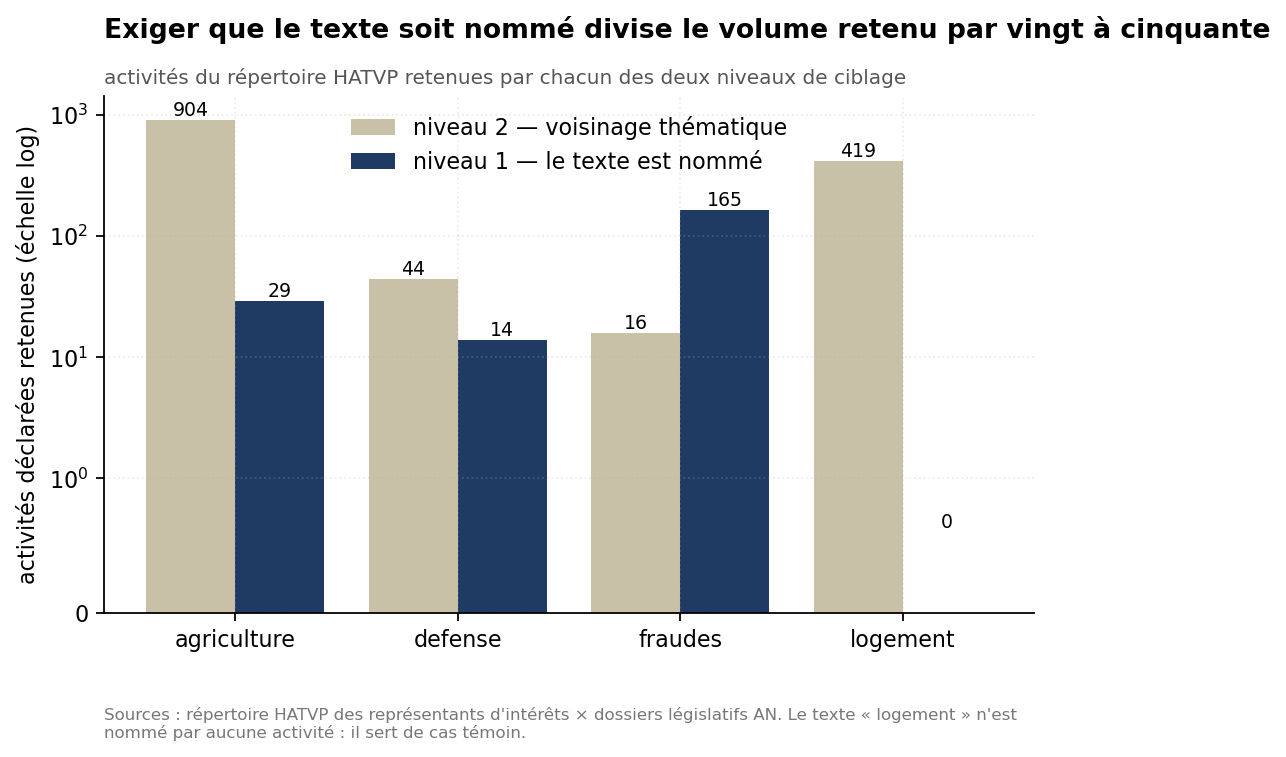
\includegraphics[width=0.78\textwidth]{../reports/figures/02_intensite_lobbying.png}
\caption{Exiger que le texte soit nommé divise le volume retenu par vingt à cinquante.
Noter le texte \texttt{logement} : 419 activités thématiquement proches, \textbf{zéro} qui
le nomme.}
\end{figure}

\begin{jargon}[Pourquoi aucune « similarité approximative » au niveau 1]
Une version intermédiaire comparait le titre du texte à l'objet déclaré avec un score de
similarité partielle (\texttt{partial\_token\_set\_ratio}). Elle retenait
\textbf{11\,170 activités sur 11\,501}, dont des déclarations sur le budget de la sécurité
sociale pour la loi agricole.

C'est le comportement normal de ce score : il renvoie 100 dès que les mots de la référence
apparaissent quelque part dans la cible, même dispersés. \textbf{Le flou est le bon outil
pour comparer deux titres} (le rapprochement précédent). \textbf{C'est le mauvais outil
pour chercher un titre dans un paragraphe.}

Le même piège s'est reproduit plus tard sur une autre source --- il y rattachait tout à
« Allocution du Président d'âge » avec un score de 100. Il est maintenant couvert par un
test automatique, pour qu'il ne se reproduise pas une troisième fois.
\end{jargon}

\subsection{L'audit manuel : le chiffre qui compte}

60~paires tirées au sort, 20 par niveau, relues une à une. Les cas plausibles mais
invérifiables sont annotés « incertain » et \textbf{exclus} du calcul : les ranger d'un
côté ou de l'autre fabriquerait le résultat.

\begin{center}
\small
\begin{tabular}{@{}lrrrr@{}}
\toprule
\textbf{Niveau} & \textbf{Relues} & \textbf{Vrais ciblages} & \textbf{Incertains} & \textbf{Précision} \\
\midrule
1 --- le texte est nommé & 20 & 20 & 0 & \textbf{100~\%} \\
2 --- voisinage thématique & 20 & 1 & 4 & \textbf{6~\%} \\
0 --- écartées & 20 & 0 & 0 & --- (aucun oubli) \\
\bottomrule
\end{tabular}
\end{center}

Sur l'échantillon, le niveau~1 a un \textbf{rappel de 95~\%} : une seule activité
réellement ciblante lui a échappé, parce qu'elle écrivait « PJL Agricole », forme absente
de la liste d'abréviations. L'abréviation a été ajoutée, ce qui a capturé trois activités
supplémentaires, toutes vérifiées et correctes. \emph{Cette itération est documentée plutôt
que masquée} : le seuil n'a pas été réglé sur le résultat final, une erreur identifiée a
été corrigée.

\begin{encadre}[À retenir pour la soutenance]
L'échantillon est \textbf{stratifié}, pas aléatoire simple : on a tiré 20~paires par
niveau pour pouvoir juger chaque niveau. Ces précisions valent donc \emph{par strate} et ne
s'extrapolent pas en un taux global. Si on te demande « quelle est la précision globale de
votre matching ? », la bonne réponse est : « la question n'a pas de sens telle quelle, nous
mesurons une précision par niveau, et voici pourquoi ».
\end{encadre}

\subsection{Un contre-exemple utile : quand la source fournit la clé}

Tout n'est pas du rapprochement approximatif. Chaque acteur de l'open data de l'Assemblée
porte un champ \fichier{uri\_hatvp} qui pointe \emph{exactement} sur sa page nominative à
la HATVP. \chiffre{88~\%} des députés sont appariés par cette clé exacte, sans aucune
heuristique (les 12~\% restants n'ont pas de déclaration publiée à la date de collecte).

La leçon tient en une phrase, et elle vaut au-delà de ce projet :
\textbf{chercher la clé fournie par la source avant d'inventer la sienne.}

\newpage
% =====================================================================
\section{Construire une variable qui n'existe pas dans les données}

\subsection{Le problème}

Le répertoire HATVP dit « j'ai contacté des députés ». Il ne dit \textbf{jamais} lequel.
Une exposition individuelle au lobbying ne peut donc pas être \emph{lue} dans les données :
elle doit être \emph{construite}.

\textbf{La méthode retenue.} Pour chaque texte, on apprend un espace TF-IDF commun sur
l'union de deux corpus --- les exposés des motifs des amendements, et les objets déclarés
des lobbies qui nomment le texte --- puis on calcule les similarités cosinus.

\begin{jargon}[TF-IDF et cosinus, en deux phrases]
Le \textbf{TF-IDF} transforme un texte en vecteur de nombres : chaque mot reçoit un poids
d'autant plus fort qu'il est fréquent dans ce texte et rare dans les autres. Le
\textbf{cosinus} entre deux vecteurs mesure alors à quel point deux textes emploient le
même vocabulaire rare --- 0 s'ils n'ont rien en commun, 1 s'ils sont identiques.
\end{jargon}

\begin{alerte}[Ce que cette mesure n'est pas]
Ce n'est \textbf{pas} une mesure de contact. C'est une mesure de \textbf{convergence de
discours}, et trois lectures sont possibles, que les données ne permettent pas de
départager :
\begin{enumerate}
\item le lobby a influencé la rédaction de l'amendement ;
\item le lobby a ciblé un député \emph{déjà convaincu} --- c'est la lecture la plus
  fréquente dans la littérature sur le lobbying, et elle suffit à produire la corrélation
  sans aucune influence ;
\item les deux emploient le vocabulaire technique du secteur, sans lien.
\end{enumerate}
C'est pourquoi le mot « influence » n'apparaît jamais sans « déclarée » dans les titres
de figures.
\end{alerte}

\subsection{Le test placebo}

Rien ne garantit a priori que la mesure capte du \emph{sectoriel} plutôt que du
\emph{style}. On calcule donc, pour chaque amendement, une \textbf{seconde} proximité :
celle aux demandes déclarées des lobbies d'un \emph{autre} texte de l'étude. Si les deux se
valaient, la mesure ne capterait que « cet amendement est écrit en français administratif
dense », et il faudrait tout jeter.

Détail technique qui a son importance : les deux corpus sont ramenés à la \textbf{même
taille} par tirage à graine fixe, parce que le maximum d'une similarité sur $N$ documents
croît mécaniquement avec $N$. Sans cette correction, le témoin « gagnait » sur la défense
simplement parce que son corpus comptait 165~objets contre 14.

\begin{figure}[htbp]
\centering
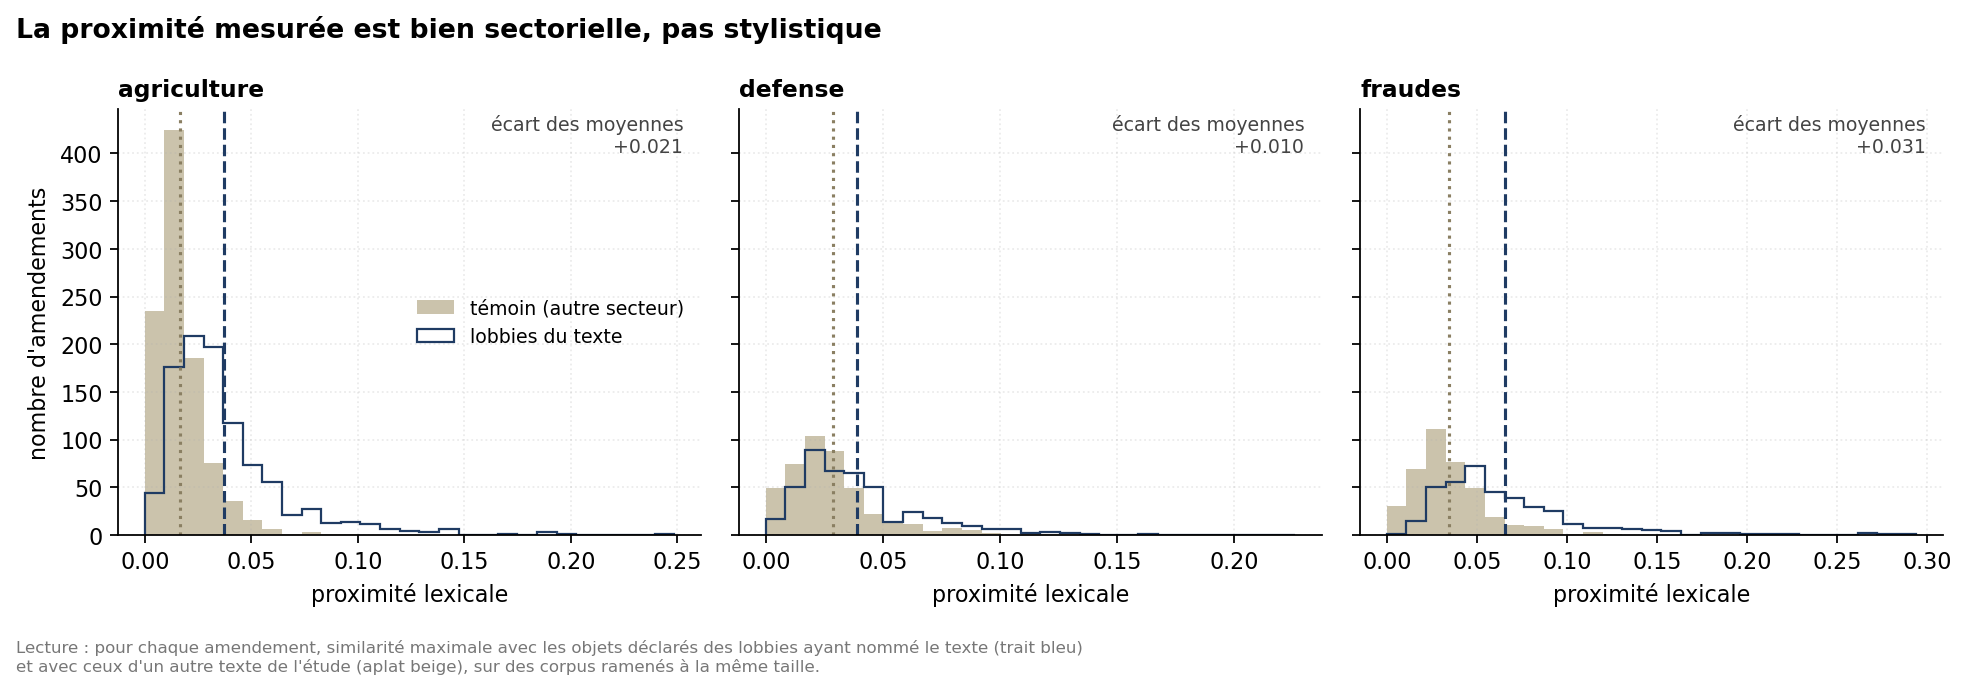
\includegraphics[width=\textwidth]{../reports/figures/10_test_placebo.png}
\caption{La proximité réelle domine le témoin sur les trois textes. La mesure capte bien
quelque chose de sectoriel --- ce qui ne dit toujours rien d'une influence.}
\end{figure}

\newpage
% =====================================================================
\section{Les résultats}

Quatre régressions logistiques, dans un ordre qui est un argument et pas un catalogue.

\begin{jargon}[Lire une régression logistique]
Elle estime la probabilité d'un événement binaire (voter « pour », être adopté\ldots) en
fonction de plusieurs variables. On lit surtout deux choses :
l'\textbf{odds ratio} (à droite de 1 : l'événement devient plus probable ; à gauche :
moins) et la \textbf{p-value} (en dessous de 0,05, on considère par convention que l'effet
n'est pas dû au hasard).

Ici tous les écarts-types sont \textbf{groupés par député} : un même député apparaît dans
des centaines de scrutins, ses erreurs sont corrélées, et des écarts-types classiques
seraient artificiellement petits --- donc des p-values artificiellement bonnes.
\end{jargon}

\subsection{Le vote final : un échec informatif}

\begin{figure}[htbp]
\centering
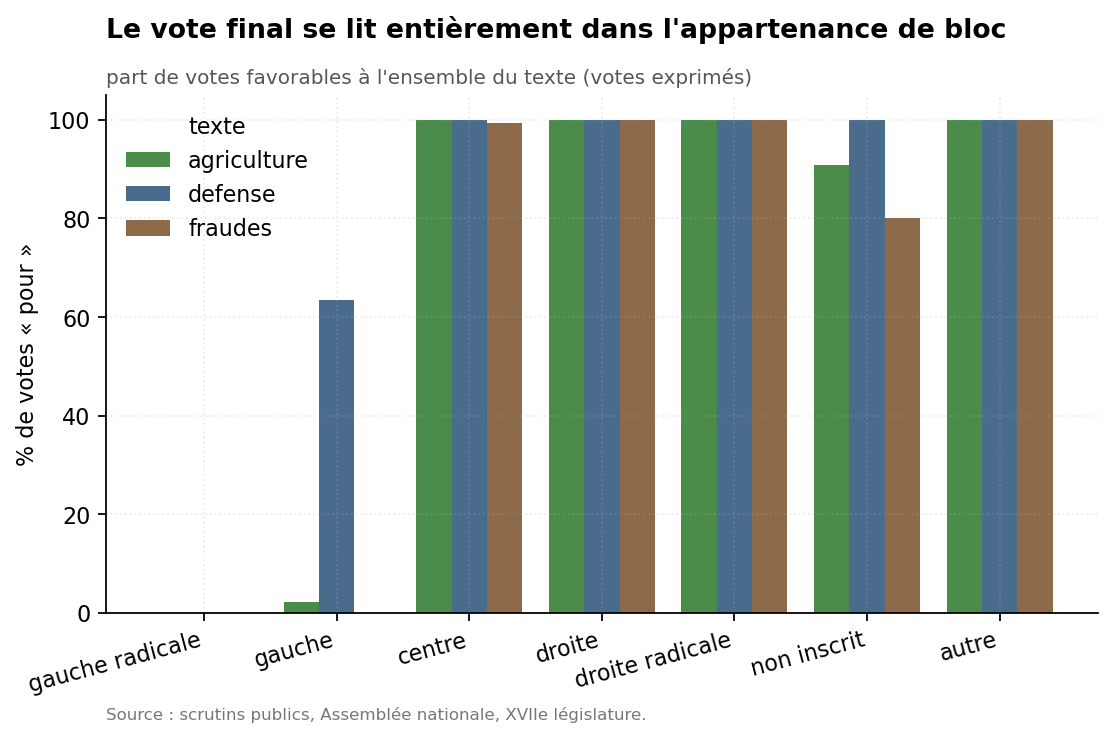
\includegraphics[width=0.82\textwidth]{../reports/figures/04_votes_par_bloc.png}
\caption{Le vote sur l'ensemble du texte se lit entièrement dans l'appartenance de bloc.}
\end{figure}

La règle « chaque député vote comme la majorité de son bloc » se trompe sur :

\begin{center}
\small
\begin{tabular}{@{}lrrr@{}}
\toprule
\textbf{Texte} & \textbf{Votes exprimés} & \textbf{Erreurs} & \textbf{Exactitude} \\
\midrule
agriculture & 547 & 3 & 99,5~\% \\
defense & 562 & 37 & 93,4~\% \\
fraudes & 557 & 3 & 99,5~\% \\
\bottomrule
\end{tabular}
\end{center}

Conséquence directe : un modèle logistique avec effets fixes de bloc \textbf{ne converge
pas}, parce que cinq blocs sur sept votent à 0~\% ou 100~\%. Le code le détecte et le dit,
au lieu d'afficher des écarts-types astronomiques. \emph{Ce n'est pas un bug à contourner,
c'est le résultat} : il n'y a plus de variance à expliquer à ce niveau. Il faut descendre
d'un cran.

\subsection{La dissidence sur les amendements}

Sur les \chiffre{970} scrutins d'amendements des trois textes, \chiffre{4,3~\%} des
89\,472 votes s'écartent de la position majoritaire du groupe --- et 74~\% des députés
dissident au moins une fois sur la loi agricole. Voilà la variance qu'on cherchait.

\begin{figure}[htbp]
\centering
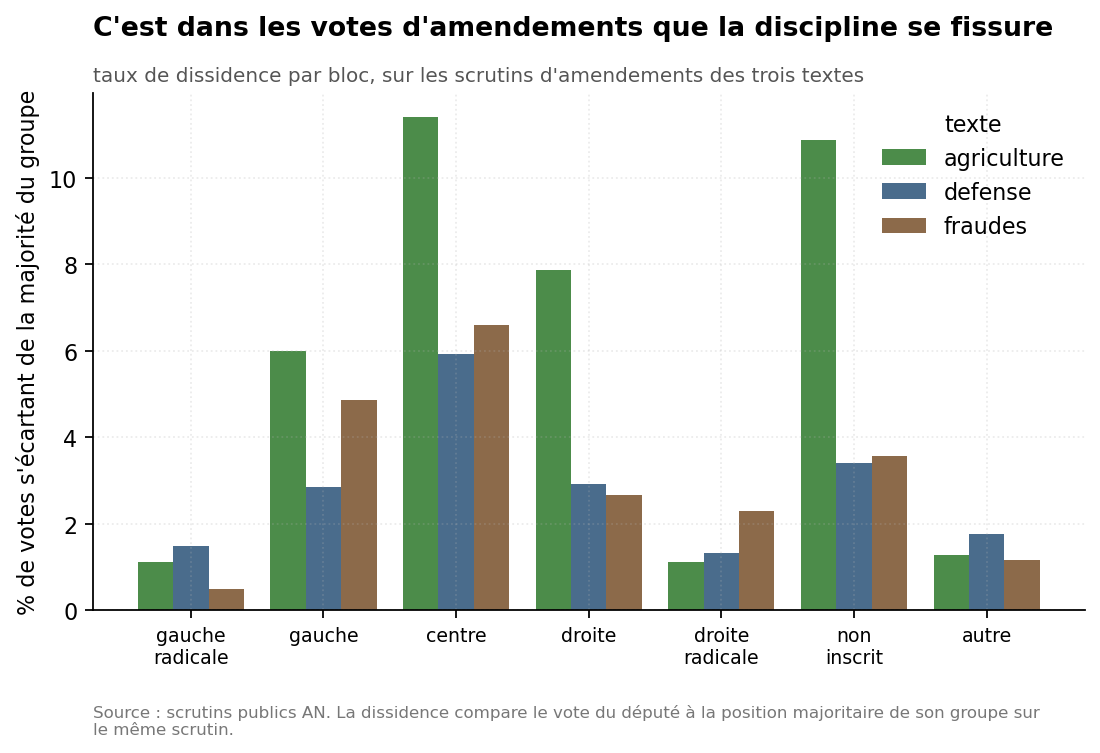
\includegraphics[width=0.8\textwidth]{../reports/figures/05_dissidence_par_bloc.png}
\caption{C'est dans les votes d'amendements que la discipline se fissure.}
\end{figure}

Effets marginaux moyens, en points de probabilité :

\begin{center}
\small
\begin{tabular}{@{}lrr@{}}
\toprule
\textbf{Variable} & \textbf{Effet} & \textbf{p} \\
\midrule
proximité lexicale avec les lobbies ($+1$ écart-type) & $+0{,}34$ pt & 0,080 \\
intérêt sectoriel déclaré & $+0{,}72$ pt & 0,082 \\
a déposé un amendement sur le texte & $-1{,}09$ pt & \textbf{0,031} \\
ruralité de la circonscription ($+1$ écart-type) & $+0{,}00$ pt & 0,982 \\
membre de la commission saisie au fond & $-0{,}20$ pt & 0,494 \\
\bottomrule
\end{tabular}
\end{center}

\textbf{Lecture.} Les deux variables liées au lobbying vont dans le sens attendu mais
\textbf{ne sont pas significatives} au seuil de 5~\%. \emph{On ne conclut pas à un effet.}
Et il faut regarder l'ordre de grandeur : $+0{,}34$~point sur un taux de base de 4,3~\%,
soit environ 8~\% de hausse relative, à comparer aux $+5$ à $+8$~points de l'appartenance
de bloc.

Le seul effet net est négatif, et peu surprenant : un député qui dépose des amendements sur
un texte dissidente \emph{moins}. Déposer des amendements est plutôt un marqueur
d'investissement dans la ligne de son groupe.

\subsection{L'adoption des amendements, et ce que le placebo révèle}

Changement d'unité d'observation : l'amendement lui-même. On ne garde que les
\chiffre{1\,145} amendements \emph{tranchés} (adoptés ou rejetés) --- un amendement retiré
ou tombé n'a pas été jugé sur son contenu.

\begin{center}
\small
\begin{tabular}{@{}lrrr@{}}
\toprule
\textbf{Mesure} & \textbf{Odds ratio} & \textbf{IC 95~\%} & \textbf{p} \\
\midrule
proximité aux lobbies du texte & 1,01 & [0,86 ; 1,20] & 0,891 \\
proximité aux lobbies d'un autre texte (témoin) & 0,77 & [0,62 ; 0,95] & \textbf{0,015} \\
\bottomrule
\end{tabular}
\end{center}

\begin{bon}[Pourquoi ce résultat est le plus intéressant du projet]
La proximité aux lobbies du texte n'a \textbf{aucun effet} sur l'adoption. En revanche le
\textbf{témoin} est significativement \emph{négatif} : un amendement dont le vocabulaire
ressemble aux demandes d'un \emph{autre} secteur a moins de chances d'être adopté.

Sans le placebo, on aurait conclu « pas d'effet » et on serait passé à côté de ce que la
mesure capte réellement : \textbf{elle sépare les amendements dans le sujet de ceux qui en
sortent}, et les amendements hors sujet sont rejetés. C'est rassurant sur le fonctionnement
parlementaire, et instructif sur ce que mesure vraiment un cosinus TF-IDF.
\end{bon}

Ce qui prédit réellement l'adoption reste l'appartenance politique : par rapport au centre,
les odds d'adoption sont divisés par~3 à droite et par~15 à la gauche radicale.

\subsection{Le résultat le mieux identifié : les intérêts déclarés}

Jusqu'ici, toutes les mesures d'exposition reposaient sur une inférence. Il existe pourtant
une information \textbf{déclarée par le député lui-même} et jamais inférée : ses intérêts
privés (anciens employeurs, participations, fonctions de direction, bénévolat).

Encore faut-il la nettoyer. Première découverte : \chiffre{51~\% de doublons}. Un député qui
dépose une déclaration initiale puis une déclaration modificative voit ses intérêts
inchangés recopiés à l'identique. Les compter deux fois aurait gonflé mécaniquement les
députés les plus actifs administrativement --- exactement le contraire de ce qu'on cherche.

\begin{figure}[htbp]
\centering
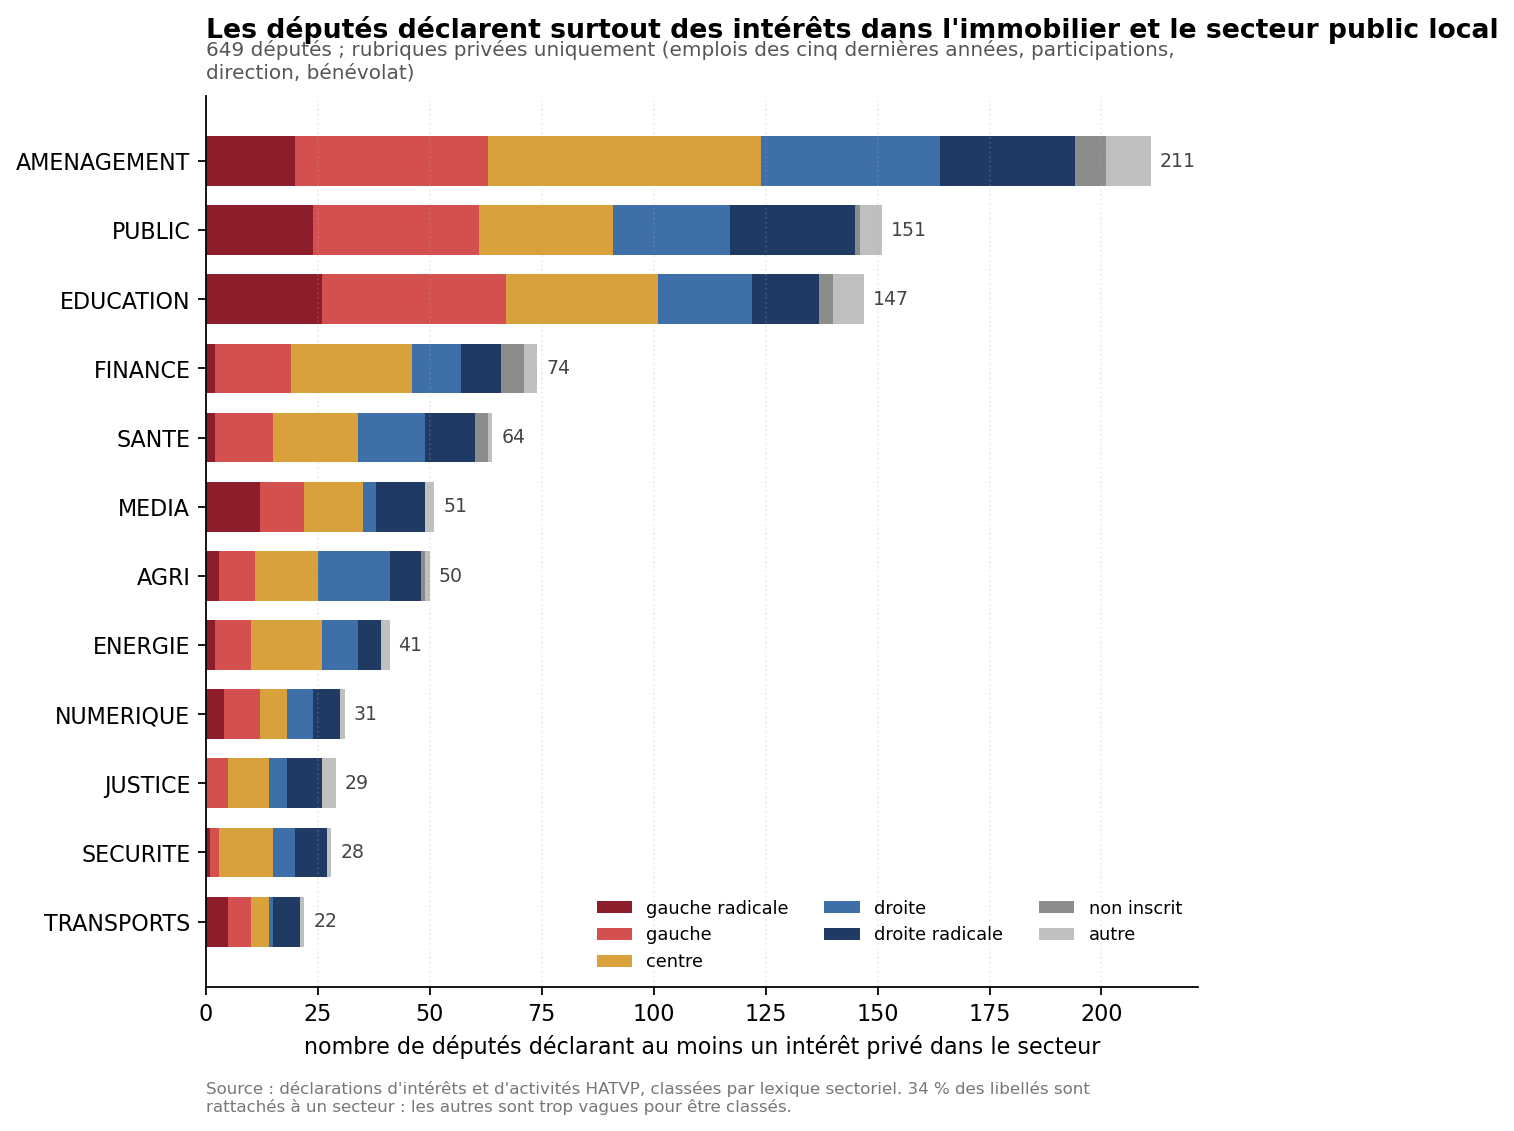
\includegraphics[width=0.84\textwidth]{../reports/figures/13_secteurs_interets.png}
\caption{Le classement sectoriel repose sur un lexique court et lisible ; il ne rattache
que 34~\% des libellés, « autoentrepreneur » ou « SCI familiale » ne disant rien du
secteur. C'est une limite, pas un détail.}
\end{figure}

\begin{figure}[htbp]
\centering
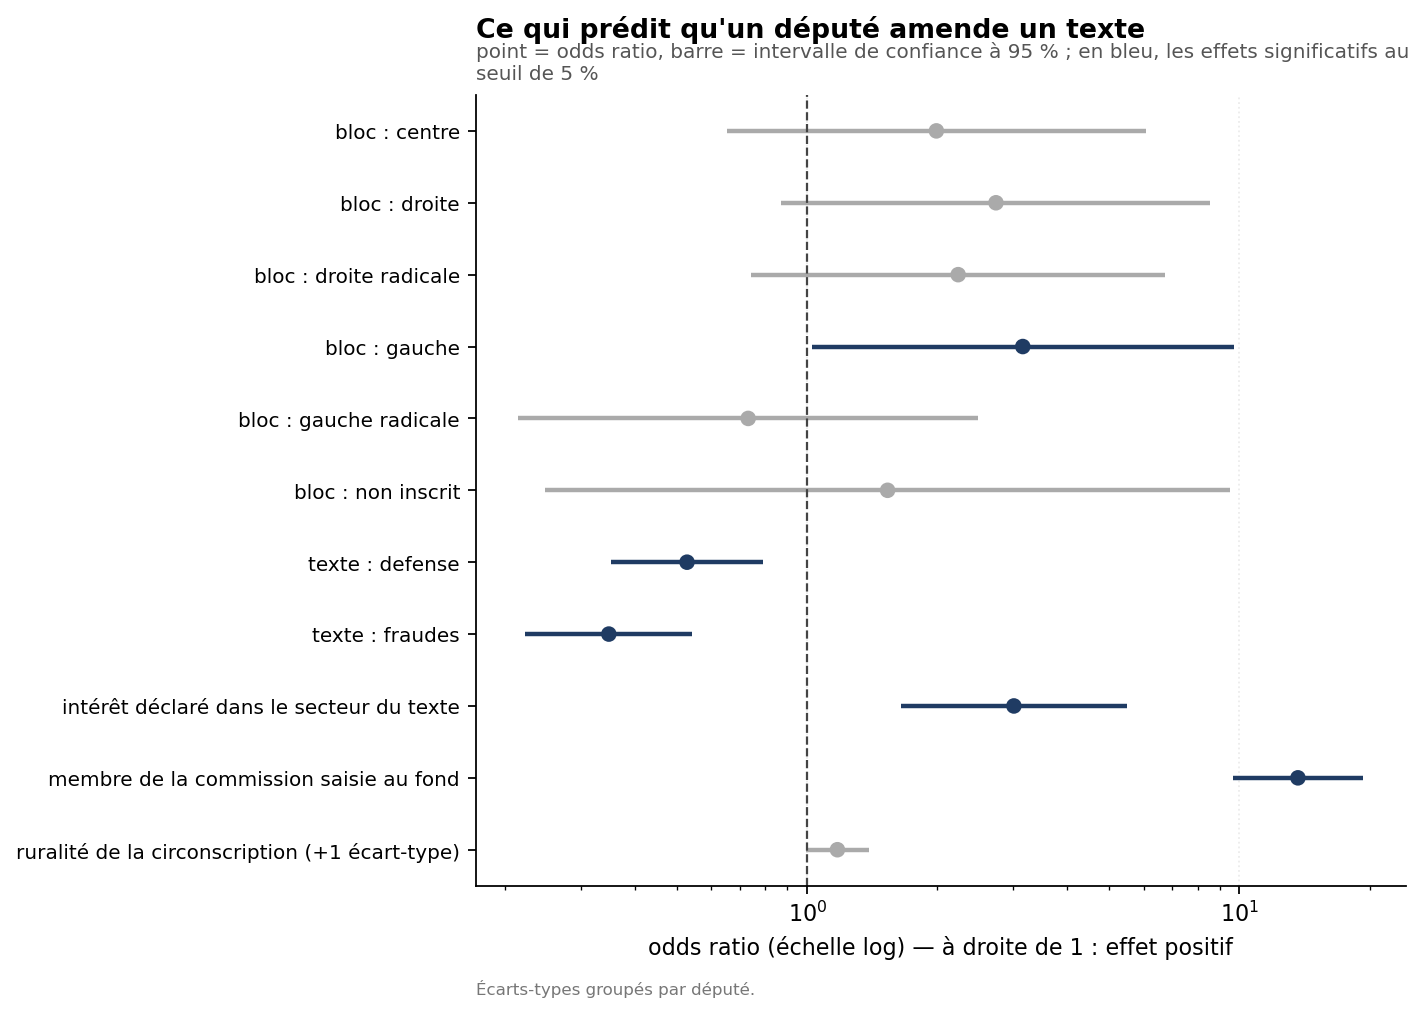
\includegraphics[width=0.84\textwidth]{../reports/figures/12_coefficients_specialisation.png}
\caption{Un député qui déclare un intérêt privé dans le secteur d'un texte a environ trois
fois plus de chances d'y déposer un amendement ; un membre de la commission saisie au fond,
quatorze fois plus.}
\end{figure}

\begin{encadre}[Comment formuler ce résultat sans se tromper]
C'est la seule relation du projet qui n'exige \textbf{aucune inférence} : les intérêts sont
déclarés par le député lui-même, et le dépôt d'un amendement est un fait.

Mais ce n'est \textbf{pas} une mise en cause. Un ancien agriculteur qui siège en commission
des affaires économiques et amende la loi agricole fait exactement ce pour quoi il a été
élu. La frontière entre \textbf{spécialisation} et \textbf{conflit d'intérêts} n'est pas
dans ces données : elle est dans le \emph{sens} de l'amendement, que le TF-IDF ne voit pas.

C'est probablement la question que le correcteur posera. La réponse est celle-là.
\end{encadre}

\newpage
% =====================================================================
\section{Robustesse : ce qui se passe quand on change les choix arbitraires}

Trois choix du projet n'ont aucune justification théorique et ont été faits à la main. Un
résultat qui dépend d'un de ces choix n'est pas un résultat.

\subsection{La largeur de la fenêtre temporelle}

Le répertoire ne date les activités qu'à l'année. On considère donc qu'une activité peut
concerner un texte si son exercice recouvre la fenêtre de débat, élargie de six mois ---
six mois étant un chiffre \emph{choisi}, pas mesuré.

\begin{figure}[htbp]
\centering
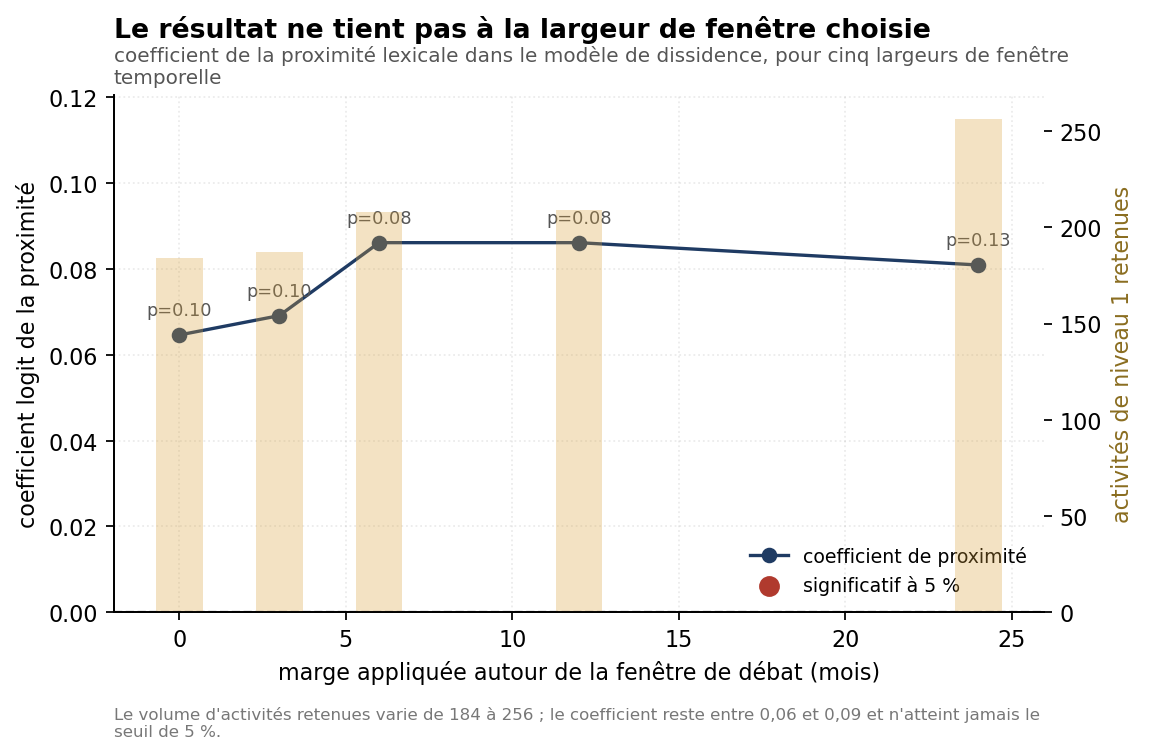
\includegraphics[width=0.82\textwidth]{../reports/figures/14_sensibilite_fenetre.png}
\caption{Le volume d'activités retenues passe de 184 à 256 selon la fenêtre, mais le
coefficient reste entre 0,06 et 0,09 et n'atteint jamais le seuil de 5~\%. Le non-résultat
n'est pas un artefact de ce choix.}
\end{figure}

\subsection{La façon de mesurer}

\begin{center}
\small
\begin{tabular}{@{}lrrr@{}}
\toprule
\textbf{Variante} & \textbf{Odds ratio} & \textbf{p} & \textbf{Conclusion} \\
\midrule
proximité = maximum & 1,09 & 0,081 & non significatif \\
proximité = moyenne des 5 plus proches & 1,07 & 0,236 & non significatif \\
\midrule
intérêt = vocabulaire du texte & 3,01 & 0,0003 & significatif \\
intérêt = classement sectoriel & 1,70 & 0,054 & limite \\
\bottomrule
\end{tabular}
\end{center}

\begin{alerte}[Ce qui tempère le résultat de la section précédente]
Les deux façons de repérer un intérêt sectoriel s'accordent à 93~\% --- mais sur une
variable aussi rare, l'accord brut est trompeur : le \textbf{kappa de Cohen} vaut
\chiffre{0,45}, soit un accord seulement modéré.

L'effet reste positif et de même sens avec les deux mesures, mais son ampleur passe d'un
odds ratio de \textbf{3,0} à \textbf{1,7}, et sa p-value de 0,0003 à 0,054.

La conclusion honnête est donc : \emph{le sens de la relation est robuste, son ampleur ne
l'est pas.} Mieux vaut annoncer le bas de la fourchette.
\end{alerte}

\subsection{Le déterminisme}

Deux sources d'aléa existent dans le projet : le tirage de l'échantillon d'audit et le
sous-échantillonnage du corpus placebo. Les deux sont à graine fixe --- encore faut-il le
vérifier, parce qu'une graine oubliée ne se voit jamais sur une seule exécution. Le
pipeline recalcule donc trois tables deux fois de suite et compare leurs empreintes
SHA-256. Les trois sont identiques.

\newpage
% =====================================================================
\section{Un détour qui vaut le coup : les déports}

Un \textbf{déport} est la décision d'un député de ne pas prendre part à un vote en raison
d'un intérêt personnel. C'est, dans tout le paysage de données exploré par ce projet,
\textbf{le seul endroit où un député, un intérêt privé et un texte précis sont nommés
ensemble}. Le répertoire HATVP ne nomme jamais le député approché ; les déclarations
d'intérêts ne nomment aucun texte. Ici, les trois sont réunis.

Mais il y en a \chiffre{59} depuis 2017, dont 9 pour la législature en cours. Aucune
statistique n'est possible : c'est une source qualitative, et un \textbf{point de
vérification} du reste de la chaîne --- les scrutins étant nominatifs, un déport annoncé
est contrôlable ligne à ligne.

Deux limites apparaissent immédiatement, et elles sont instructives :
\begin{itemize}
\item la plupart des déports visent \textbf{certains articles}, pas le texte entier ; on ne
  peut donc rien conclure au niveau du dossier, le député ayant le droit de voter sur tout
  le reste ;
\item deux références (« Articles de loi ayant trait aux assurances\ldots ») ne nomment
  aucun texte identifiable, et restent volontairement non rattachées --- inventer un
  rattachement serait pire que l'absence.
\end{itemize}

Un seul déport est vérifiable au niveau du dossier : un député déclarant être
« en disponibilité » d'un groupe industriel de défense, et se déportant de l'intégralité
du projet de loi de programmation militaire. Sur les \chiffre{292} scrutins du dossier
postérieurs à ce déport, il n'apparaît dans le détail nominatif que pour
\textbf{un seul vote} --- celui sur l'ensemble du texte issu de la commission mixte
paritaire.

\begin{encadre}[Ce que les données disent, et où elles s'arrêtent]
Elles disent : 291 scrutins sans position enregistrée, 1 vote exprimé. Elles ne disent
\textbf{pas} si c'est un oubli, un changement de situation, ou une lecture du déport qui
en exclut le vote final. Il n'y a aucune mise en cause à tirer de là.

Ce qu'il faut en retenir pour le projet est ailleurs : un engagement public \textbf{peut}
être vérifié ligne à ligne dès lors que la source nomme à la fois la personne et le texte.
C'est précisément ce qui manque au répertoire des lobbies, et c'est pour ça que tout le
reste du projet repose sur des inférences.
\end{encadre}

\newpage
% =====================================================================
\section{Ce que le projet ne dit pas}

Par ordre de gravité. C'est la section que le correcteur lira le plus attentivement, et
c'est elle qui vaut des points.

\begin{enumerate}
\item \textbf{Le répertoire HATVP est autodéclaratif.} Une organisation qui ne déclare rien
  est invisible. Transparency International et l'Observatoire des multinationales
  contestent régulièrement l'exhaustivité du registre. On mesure le lobbying
  \emph{déclaré}, qui est un sous-ensemble inconnu du lobbying réel.
\item \textbf{Pas de datation fine.} Une activité est rattachée à un exercice annuel ; la
  fenêtre de débat est élargie de six mois de part et d'autre, ce qui est arbitraire ---
  mais testé (section précédente).
\item \textbf{Causalité : aucune.} La corrélation mesurée est compatible avec l'absence
  totale d'influence.
\item \textbf{Rappel faible au niveau 1.} Une organisation qui décrit son action sans
  nommer le texte est perdue. Le projet préfère 208 rattachements sûrs à 1\,383 douteux,
  mais c'est un arbitrage, pas une vérité.
\item \textbf{La proximité TF-IDF est purement lexicale.} Elle ne voit pas que deux
  formulations opposées peuvent partager tout leur vocabulaire : un amendement qui
  \emph{interdit} une substance et une demande de lobby qui la \emph{réautorise} se
  ressemblent beaucoup pour un cosinus. C'est la limite la plus sérieuse du projet.
\item \textbf{Une seule législature.} La XVII\ieme{} est marquée par une fragmentation
  politique inhabituelle ; les taux de dissidence ne sont pas transposables.
\end{enumerate}

% =====================================================================
\section{L'organisation du code}

Neuf modules, un par étape du raisonnement. Le notebook ne fait qu'appeler des fonctions :
aucune logique n'y est écrite, ce qui est explicitement demandé par les consignes
(« pas de copier-coller de cellule, préférez des fonctions »).

\begin{center}
\small
\begin{tabular}{@{}lp{0.62\textwidth}@{}}
\toprule
\textbf{Module} & \textbf{Rôle} \\
\midrule
\fichier{config.py} & chemins, URL des sources, textes étudiés, nomenclatures \\
\fichier{collect.py} & téléchargement idempotent et manifeste de provenance \\
\fichier{parse\_an.py} & mise à plat de l'open data Assemblée \\
\fichier{parse\_hatvp.py} & mise à plat du répertoire et des déclarations HATVP \\
\fichier{matching.py} & rapprochement des bases et sa validation chiffrée \\
\fichier{features.py} & variables d'analyse, proximité lexicale, placebo \\
\fichier{models.py} & les quatre régressions \\
\fichier{quality.py} & 24 contrôles de qualité des données \\
\fichier{robustesse.py} & sensibilité aux choix arbitraires, déterminisme \\
\fichier{viz.py} & les 18 figures \\
\fichier{pipeline.py} & orchestration : \fichier{python -m lobbynomics.pipeline} \\
\bottomrule
\end{tabular}
\end{center}

\subsection{Les commandes utiles}

\begin{center}
\small
\begin{tabular}{@{}lp{0.58\textwidth}@{}}
\toprule
\textbf{Commande} & \textbf{Effet} \\
\midrule
\fichier{make pipeline} & la chaîne complète, de l'URL aux figures \\
\fichier{make rapide} & tout sauf le téléchargement et la mise à plat ($\approx$~1~min) \\
\fichier{make tests} & les 58 tests \\
\fichier{make rapport} & exécute le notebook de bout en bout \\
\fichier{make qualite} & les contrôles de qualité seuls \\
\bottomrule
\end{tabular}
\end{center}

Une \textbf{intégration continue} GitHub Actions lance les tests à chaque poussée, sur
Python 3.11 et 3.12. Elle ne télécharge aucune donnée : une CI qui dépend de 700~Mo
d'open data tombe en panne le jour où une source change d'URL, pour une raison qui n'a
rien à voir avec le code.

% =====================================================================
\section{Préparer la soutenance}

Les questions probables, et ce qu'il faut répondre.

\begin{center}
\small
\begin{longtable}{@{}p{0.37\textwidth}p{0.58\textwidth}@{}}
\toprule
\textbf{Question} & \textbf{Réponse} \\
\midrule
\endhead
« Vous ne trouvez rien, alors ? » & Sur les lobbies, non, et c'est dit. Le projet mesure
surtout le \emph{prix du rapprochement} entre bases : 99,5~\% de précision ici, 6~\% pour
une règle plausible qu'on a dû jeter. C'est ça le résultat. \\
« Pourquoi pas de régression sur le vote final ? » & Parce qu'elle ne converge pas : cinq
blocs sur sept votent à 0 ou 100~\%. Le modèle sépare parfaitement les données. On le
montre, on l'explique, et on change de niveau d'observation. \\
« Comment savez-vous que votre matching est bon ? » & Deux façons : les 2\,608 scrutins à
lien explicite servent de vérité terrain gratuite ; et 60~paires HATVP ont été relues une
à une, avec le détail des verdicts dans le dépôt. \\
« Pourquoi avoir choisi ces trois textes ? » & Lobbying documenté, volumes suffisants, et
trois secteurs différents. Le quatrième texte est gardé comme témoin négatif. \\
« C'est quoi votre variable d'exposition, exactement ? » & Une convergence de vocabulaire,
pas un contact. Le répertoire ne nomme jamais le député. On le dit dans chaque titre de
figure. \\
« Et la causalité ? » & Aucune. Un lobby cible d'abord les députés déjà convaincus ; la
corrélation serait la même sans aucune influence. \\
« Pourquoi un test placebo ? » & Pour vérifier que la mesure capte du sectoriel et pas du
style. Et il a appris quelque chose : c'est le témoin qui est significatif, pas la vraie
mesure. \\
« Votre projet est-il reproductible ? » & Une commande, un manifeste de provenance avec
empreintes SHA-256, 58 tests, une CI, et une vérification que deux exécutions donnent
exactement les mêmes nombres. \\
\bottomrule
\end{longtable}
\end{center}

% =====================================================================
\section{Ce qu'il te reste à faire}

\begin{enumerate}
\item \textbf{Faire valider le sujet} par la chargée de TD du cours. C'est
  explicitement exigé.\footnote{Son adresse figure dans le courriel du 22 septembre 2026 ;
  elle n'est pas recopiée ici, ce dépôt étant public.}
\item \textbf{T'inscrire sur le Google Sheet} de constitution des groupes (2 à 3 personnes).
\item \textbf{Créer le dépôt GitHub public} et y pousser \emph{progressivement}.
  L'historique de version est noté : les dépôts constitués d'un seul envoi sont pénalisés.
  Le dépôt local contient déjà neuf commits thématiques pour démarrer.
\item \textbf{Confirmer les dates} de rendu et de soutenance : la page du cours affiche
  encore « XX décembre 2026 » et « XX janvier » au 2 octobre.
\item \textbf{Relire l'audit manuel} (\fichier{data/processed/audit\_ciblage\_a\_annoter.csv}).
  Les 60~verdicts y sont, avec un commentaire pour chaque cas discutable. C'est ton nom qui
  sera dessus : si tu n'es pas d'accord avec un verdict, change-le, le pipeline recalcule
  les précisions automatiquement.
\item \textbf{Lire \fichier{docs/methode.md}} avant la soutenance : c'est la version longue
  de ce document, avec les impasses détaillées.
\end{enumerate}

\subsection*{Les pistes si vous voulez aller plus loin}

\begin{itemize}
\item \textbf{Les textes budgétaires} (projet de loi de finances, budget de la sécurité
  sociale), où le lobbying déclaré est de très loin le plus dense --- et où le
  rattachement des scrutins est le plus difficile, donc le plus intéressant.
\item \textbf{Un modèle de phrases} à la place du TF-IDF, pour capter l'opposition
  sémantique que le cosinus lexical ignore.
\item \textbf{Le sens des amendements} : c'est le vrai chaînon manquant entre
  spécialisation et capture, et aujourd'hui personne ne le mesure proprement.
\end{itemize}

\vfill
\begin{center}
\color{cGris}\small
Projet réalisé avec l'aide d'un assistant de code, ce que les consignes du cours
autorisent explicitement --- à condition de comprendre et d'assumer ce qui est rendu.
C'est l'objet de ce document.
\end{center}

\end{document}
